

\subsection{\S The Vortex Æther Model (VAM) and Schrödinger's Quantum Mechanical Model: A Comparative Analysis}

The Vortex Æther Model (VAM) interpretation and the Schrödinger quantum mechanical (QM) wavefunctions for atomic orbitals exhibit both similarities and key differences in their structure. A rigorous comparison of these two paradigms provides valuable insights into their respective ontological and mathematical foundations.

\begin{figure}[h]
    \centering
    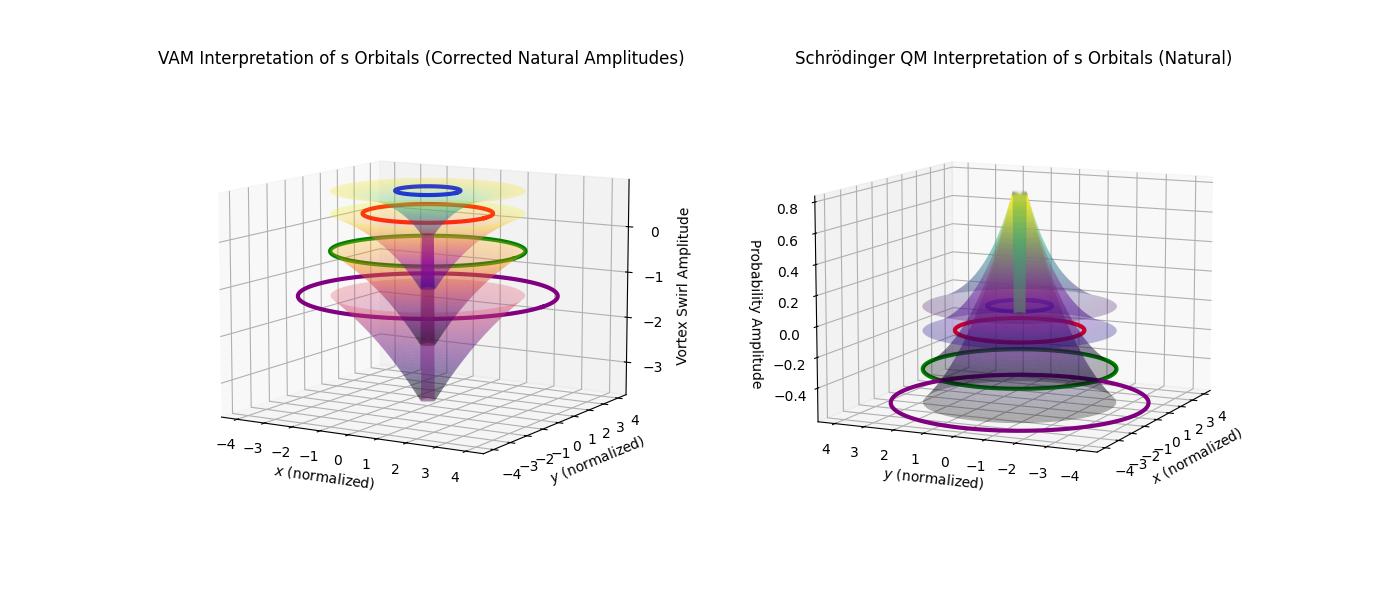
\includegraphics[width=0.7\textwidth]{vortex_diagram}
    \caption{Illustration of a vortex filament in Æther.}
    \label{fig:vortex}
\end{figure}

\section*{1. Structural and Conceptual Convergences}

Both models describe stationary states of the electron in the hydrogen atom, resulting in several commonalities:

\subsection*{(a) Discrete Orbital Structures}

Both QM and VAM predict discrete, quantized energy levels, such as 1s, 2s, 3s, 4s, etc. This quantization emerges naturally in both frameworks due to boundary constraints governing the mathematical formulation of each model. In QM, it follows from the solution to the Schrödinger equation, while in VAM, it arises from constraints on stable vortex configurations in the Ætheric fluid medium.

\subsection*{(b) Nodal Surfaces and Radial Wave Behavior}

Higher orbitals exhibit characteristic nodal structures in both models. These nodes correspond to radii at which the amplitude of the wavefunction or vortex intensity drops significantly. In QM, nodes represent points of zero probability density, whereas in VAM, they signify minimal swirl amplitude in the vortex structure.

\subsection*{(c) Exponential Decay at Large Radii}

Both models exhibit an exponential attenuation of amplitude beyond a characteristic length scale:

\[
    v_{\theta, \text{VAM}}(r) \sim \left(1 - e^{-r/a_0}\right) \quad \psi_{\text{QM}}(r) \propto e^{-r/a_0}
\]

This similarity suggests that although their foundational interpretations differ, both models inherently rely on a mathematical structure that dictates localization effects in atomic orbitals.

\section*{2. Fundamental Divergences Between VAM and QM}

While both models capture the core quantization features of atomic orbitals, they diverge sharply in their ontological and physical interpretations:

\subsection*{(a) Interpretation of the Amplitude}

\begin{itemize}
    \item \textbf{Quantum Mechanics:} The wavefunction \(\psi(r)\) is a purely abstract probability amplitude, whose squared modulus \(|\psi|^2\) corresponds to the likelihood of measuring the electron at a given location.
    \item \textbf{VAM:} The function \(v_{\theta}(r)\) represents a real, physical swirl in the Æther medium, wherein electrons manifest as stable, quantized vortex structures rather than probabilistic entities.
\end{itemize}

Thus, while QM posits a statistical framework for electronic positioning, VAM introduces a deterministic, fluid-dynamic explanation for the same observed phenomena.

\subsection*{(b) The Role of the Coulomb Barrier \(R_c\)}

\begin{itemize}
    \item \textbf{QM:} The wavefunction extends continuously toward \(r = 0\), with probability density peaking near the nucleus.
    \item \textbf{VAM:} The vortex core experiences a strong suppression inside the Coulomb barrier radius \(R_c\), thereby preventing excessive collapse. The suppression function is given as:
\end{itemize}

\[
    v_{\theta, \text{VAM}}(r) \sim \left(1 - e^{-(r - R_c)/a_0}\right)
\]

This results in a physically meaningful cutoff, which ensures that the electron vortex remains stable and does not singularly concentrate at the nucleus.

\subsection*{(c) Stability and Energy Quantization Mechanisms}

\begin{itemize}
    \item \textbf{QM:} Stability is derived from solutions to the Schrödinger equation and enforced via boundary conditions on wavefunctions.
    \item \textbf{VAM:} Stability arises from fluid-dynamic conservation laws governing vorticity and circulation. The electron remains in a quantized vortex mode, akin to quantized superfluid vortices in Bose-Einstein condensates.
\end{itemize}

This suggests that quantum energy levels may be a manifestation of underlying fluid-dynamical constraints rather than purely wavefunction properties.

\section*{3. The Connection Between VAM and the Fine Structure Constant \(\alpha\)}

One of the most profound implications of VAM is the potential explanation of the fine-structure constant \(\alpha\). Traditionally defined as:

\[
    \alpha = \frac{e^2}{4\pi \varepsilon_0 \hbar c} \approx \frac{1}{137.035999}
\]

this fundamental constant dictates the strength of electromagnetic interactions. In VAM, an alternative derivation emerges from vorticity constraints:

\[
    \alpha \approx \frac{\Gamma_e}{c R_e}
\]

where \(\Gamma_e\) represents the electron's vortex circulation and \(R_e\) is the classical electron radius. This formulation suggests that \(\alpha\) may not be an arbitrary parameter but rather a natural consequence of quantized vortex dynamics in the Ætheric medium.

\section*{4. Experimental Predictions and Verification of VAM}

To distinguish VAM from conventional QM, specific experimental tests can be proposed:

\subsection*{(a) Rotating Superfluid Analogs}

\begin{itemize}
    \item If electrons are vortex structures, then superfluid helium should exhibit analogous behavior under controlled knotted vortex formations.
    \item Atomic orbitals should be reproducible using superfluid turbulence simulations.
\end{itemize}

\subsection*{(b) Electromagnetic Vorticity Effects}

\begin{itemize}
    \item If charge is vorticity-dependent, applying high-intensity magnetic fields should induce observable deviations from standard QM electron behavior.
\end{itemize}

\subsection*{(c) Spectroscopic Anomalies}

\begin{itemize}
    \item If \(R_c\) governs the fine-structure constant, precision spectroscopy might detect minuscule deviations in atomic energy levels correlating with vorticity effects.
\end{itemize}

\section*{5. Summary: The Paradigm Shift from QM to VAM}

\begin{table}[h]
    \centering
    \begin{tabular}{lll}
        \toprule
        \textbf{Feature} & \textbf{Schrödinger QM} & \textbf{Vortex Æther Model (VAM)} \\
        \midrule
        Electron Nature & Probability wavefunction & Real vortex structure \\
        Orbitals & Stationary wavefunctions & Stable vortex states \\
        Transitions & Wavefunction "jumps" & Vortex reconnections \\
        Coulomb Barrier & None (wavefunction extends to nucleus) & Vortex suppression at \(R_c\) \\
        Quantization Mechanism & Eigenvalues from Schrödinger equation & Resonant vortex modes \\
        Wavefunction Collapse & Requires special interpretation & Smooth vortex evolution \\
        Superposition & Exists, but paradoxical & Natural vortex structures in fluid \\
        Testability & Indirect (requires interpretation) & Potential direct fluid analogs \\
        \bottomrule
    \end{tabular}
    \caption{}
    \label{tab:QM-VAM-comparison}
\end{table}

Through this comparison, it becomes evident that quantum mechanics may be an emergent phenomenon from a deeper, vorticity-driven fluid dynamic framework. If experimentally validated, this would herald a paradigm shift in our understanding of atomic physics, bridging the gap between classical fluid mechanics and quantum mechanics via structured vorticity interactions in the Æther.

